\documentclass[12pt,
				openright,
				twoside,
				a4paper,
				apter=TITLE,
				section=TITLE,
				subsection=TITLE,
				chapter=TITLE,
				english,
%				french,
%				spanish,
				brazil]{abntex2}

\usepackage{lmodern}
\usepackage{mathtools} 			%Math tags
\usepackage{amsmath}
\usepackage[T1]{fontenc}		% Selecao de codigos de fonte.
\usepackage{calligra}
\usepackage[utf8]{inputenc}		% Codificacao do documento (conversão automática dos acentos)
\usepackage{indentfirst}		% Indenta o primeiro parágrafo de cada seção.
\usepackage{color}				% Controle das cores
\usepackage{graphicx}			% Inclusão de gráficos
\usepackage{microtype} % para melhorias de justificação


%\usepackage[left=3cm,right=2cm,top=3cm,bottom=2cm]{geometry}
\usepackage[table]{xcolor}
\usepackage[brazilian,hyperpageref]{backref}	 % Paginas com as citações na bibl
\usepackage[alf]{abntex2cite}	% Citações padrão ABNT



\usepackage[brazilian,hyperpageref]{backref}	 % Paginas com as citações na bibl
\usepackage[alf]{abntex2cite}	% Citações padrão ABNT
\usepackage{multirow}





\renewcommand{\backrefpagesname}{Citado na(s) página(s):~}
% Texto padrão antes do número das páginas
\renewcommand{\backref}{}
% Define os textos da citação
\renewcommand*{\backrefalt}[4]{
	\ifcase #1 %
		Nenhuma citação no texto.%
	\or
		Citado na página #2.%
	\else
		Citado #1 vezes nas páginas #2.%
	\fi}%
% ---
\newcommand{\mc}[3]{\multicolumn{#1}{#2}{#3}}

% ---
% Informações de dados para CAPA e FOLHA DE ROSTO
% ---

\titulo{Sistema de Recomendação Utilizando a Recomendação por Conteúdo}

\autor{Arthur Silva Morato}
\local{Mato Grosso do Sul - Brasil}
\data{\today}
\instituicao{%
  Fundação Universidade Federal de Mato Grosso do Sul
  \par
  Campus de Ponta Porã – MS
  \par
  Ciência da Computação – Bacharelado }
\tipotrabalho{Trabalho de Conclusão de Curso}
\orientador{Me. Daniel Matte Freitas}


\preambulo{Dissertação apresentada ao curso de graduação em Ciência da Computação da Universidade Federal de
Mato Grosso do Sul como trabalho de conclusão de curso: requisito obrigatório para colação de grau e obtenção do título de Bacharel em Ciência da Computação.}


\definecolor{blue}{RGB}{41,5,195}
\definecolor{lightgray}{gray}{0.9}

% informações do PDF
\makeatletter
\hypersetup{
     	%pagebackref=true,
		pdftitle={\@title}, 
		pdfauthor={\@author},
    	pdfsubject={\imprimirpreambulo},
	    pdfcreator={Sistema de Recomendação},
		pdfkeywords={Sistema de Recomendação}{Recomendação de Conteúdo}{Filtro Colaborativo}{Sistema de 
		Recomendação Híbrido}{Exemplos de Recomndação}{Pesquisa}, 
		colorlinks=true,       		% false: boxed links; true: colored links
    	linkcolor=black,          	% color of internal links
    	citecolor=black,        		% color of links to bibliography
    	filecolor=black,      		% color of file links
		urlcolor=black,
		bookmarksdepth=4
}
\makeatother
% --- 

% --- 
% Espaçamentos entre linhas e parágrafos 
% --- 

% O tamanho do parágrafo é dado por:
\setlength{\parindent}{1.3cm}

% Controle do espaçamento entre um parágrafo e outro:
\setlength{\parskip}{0.2cm}  % posso por também \onelineskip

% ---
% compila o indice
% ---
\makeindex
% ---


% ----
% Início do documento
\begin{document}
%\frenchspacing 


% ----------------------------------------------------------
% ELEMENTOS PRÉ-TEXTUAIS
% ----------------------------------------------------------
% \pretextual

% ---
% Capa
% ---
\begin{figure}
\centering

\includegraphics[scale=0.3]{img/logoufms}
\end{figure}
\imprimircapa
% ---

% ---
% Folha de rosto
% ---
\imprimirfolhaderosto
\imprimirtipotrabalho
\imprimirorientador
% ---



\addcontentsline{toc}{chapter}{Agradecimentos}

\begin{flushright}

\begin{minipage}[b]{13cm}
\vspace{15.01cm}
\chapter*{Agradecimentos}{
\calligra A Deus pelas bênçãos sem fim, e mais um monte de blábláblá que tenho que bolar depois!\\
A meus pais por tudo, em expecial: pela grana que me manteu todo esse tempo longe de casa.\\
A meus amigos e colegas da zuera sem fim.\\
A meus professores amados \\
A meu orientador.}

\end{minipage}
\end{flushright}

% nova página para dedicatória

\begin{flushright}
\begin{minipage}[b]{13cm}
\vspace{20.01cm}

\calligra Dedico a mim e só a mim! Vlw flw. 
Ass: Irmauzinhu

\end{minipage}
\end{flushright}
\clearpage

% ---
% Lista de imagens
% ---
\pdfbookmark[0]{\listfigurename}{lof}
\listoffigures*
\cleardoublepage
% ---

% ---
% inserir lista de tabelas
% ---
\pdfbookmark[0]{\listtablename}{lot}
\listoftables*
\cleardoublepage

\begin{siglas}
\item EXP \textit{Exemplo} 

\end{siglas}
% ---

% ---
% inserir lista de símbolos
% ---
\begin{simbolos}
  \item[$ \Gamma $] Letra grega Gama
  \item[$ \Lambda $] Lambda
  \item[$ \zeta $] Letra grega minúscula zeta
  \item[$ \in $] Pertence
\end{simbolos}
% ---

% ---
% inserir o sumario
% ---
\pdfbookmark[0]{\contentsname}{toc}
\tableofcontents*
\cleardoublepage
% ---


% ----------------------------------------------------------
% ELEMENTOS TEXTUAIS
% ----------------------------------------------------------
\textual


\frenchspacing 

\addcontentsline{toc}{chapter}{Resumo}
\chapter*{Resumo}
% ---
% Feito
% ---
Este trabalho tem como objetivo apresentar as principais técnicas sobre os Sistemas de Recomendação de conteúdo, entre muitas técnicas conhecidas, que foram derivadas ou baseadas nessas técnicas ou em outras, apresentando de forma clara todos  os seus mecanismos de funcionamento e seus respectivos resultados encontrados em trabalhos realizados anteriormente, proporcionando uma prévia dos dados obtidos em pesquisas e estudos realizados desde os primórdios do estudo sobre a recomendação e das primeiras hipóteses de recomendação por um sistema independente, onde se utiliza dados coletados para poder predizer o que poderia ser mais relevante, sendo assim, com uma maior probabilidade de acerto próximo passo, para determinado fim baseado em alguma métrica estabelecida pelo sistema, aprimorando todo o conjunto do sistema onde foi aplicado a recomendação. Para demonstração de desempenho e visualização dos resultados obtidos, será proposto neste trabalho o desenvolvimento de um framework para recomendação generalizada, onde o algoritmo passará por um processo de aprendizagem de máquina indutivo, utilizando uma base de dados que será subdividida em conjunto de teste e conjunto de aprendizagem, para poder generalizar novos casos e classificar as informações do conjunto de teste, utilizando o ``aprendizado'' obtido por meio do conjunto de aprendizagem. 


\addcontentsline{toc}{chapter}{Abstract}
\chapter*{Abstract}
% ---
% Feito
% ---
This work aims to present the main techniques on Recommender Systems, among many known techniques, which were derived from or based on such technical or other, showing clearly all its operating mechanisms and their results found in studies previously conducted providing a preview of the data obtained in surveys and studies conducted since the beginning of the study and on the recommendation of the first hypotheses recommendation by an independent system, which uses the collected data in order to predict what could be more relevant, therefore, to a higher probability of success next step for a particular purpose based on some metric established by the system, improving the whole system where the recommendation was applied. To demonstrate performance and displaying the measurement results, it is proposed in this work to develop a generalized framework for recommendation where the algorithm will go through a learning process of induction machine using a database to be divided into the test set, and learning to generalize to new cases and sort the information of the test, using the `learning 'obtained through the learning set.

\chapter{Introdução}
% ---
% Feito
% ---
A recomendação está em presente em muitos lugares e situações, uma vez que é preciso, na maioria da vezes, algum conhecimento sobre algo novo para se interessar por ele ao ponto do querer mais informações para poder confirmar o interesse, mas o primeiro obstáculo à ser derrubado é como saber o que terá nesse algo novo que poderá ser do interesse de quem ou o que, está recebendo a recomendação. Sem fazer destinção do que será recomendado, é natural o conhecimento de que todas as informações sobre um produto ou serviço é do interesse de quem está procurando, mas poder apresentar resultados baseados em suas preferências pode ser a principal etapa para definir se há realmente o interesse, ou não, proporcionando uma otimização significativa em todo o conjunto do sistema, que será refletido nos resultados que serão obtidos desse sistema. Entre pessoas, por exemplo, a preferência é ver se alguém já testou algum novo produto ou serviço, e qual foi a reação que isso proporcionol para a pessoa, para depois analisar se o novo produto pode, ou não, see bom, ou ruim, para si próprio.[1],[2].

Uma grande conquista para a tecnologia é a grande quantidade de conteúdo que pode ser compartilhado através de diversos meios de comunicação e de trafego de dados, possibilitando a propagação de informação, acessível a todas as pessoas com acesso a tecnologia, otimizando as atividades em todos os âmbitos pessoais e tecnológicas. Um grande avanço se mostra no compartilhamento em massa de informações em todas as áreas de interesses, como notícias sobre esportes, tempo, política, ou sobre estudos e pesquísas, como conseguir encontrar áreas de pesquisa e estudo que estão em destaque nos dias atuais, ou sobre alimentação, como qual restaurante poderia ser o melhor para visitar em determinada cidade, também é demonstrado avanço sobre o compartilhamento de mídias digitais, como música, áudio, filmes, texto, etc. [5]. Alguns exemplos de sistemas que conseguem recomendar CDs, livros e uma outra infinidade de produtos pelo loja online Amazon.com [3], ou filmes e suas classificações pelo site MovieLens.com [6], ou livros e críticas de livros no site barnesandnoble.com, ou artigos acadêmicos, sites, lugares para conhecer ou visitar, culinária, produtos em geral, entre outros, procurando sempre o que for melhor para oferecer aos seus usuários, que estão buscando o que for mais interessante para ele. [4], [5], [6], [7].

Descobrir o mecanismo e as funcionalidades dos algorítmos de recomendação é descobrir como a recomendação desses sistemas, citados acima, conseguem oferecer um novo produto com uma grande taxa probabilidade de que um futuro novo usuário possa gostar, e continuar recomendando com cada vez mais precisão, utilizando como parâmentro o perfil de seus usuários. Avaliando essa tarefa de recomendação como um desafio, então conseguir entender o funcionamento humano de recomendação e transformá-lo em dados através de um algorítmo que possa ``aprender'' a recomendar com a maior precisão possível, é uma provável solução para esse desafio. [2].

Neste trabalho, para uma melhor abordagem do assunto, será feita uma ampla abordagem sobre os tipos de sistemas de recomendação, alguns problemas na recomendação e suas soluções. Também é proposto nestedocumento, o desenvolvimento de um Framework para exemplificar o funcionamento de um algoritmo de recomendação, com a finalidade de visualizar os dados obtidos e verificar e comprovar a eficiência da recomendação por sistemas de Inteligência Artificial. Os resultados se encontrarão ao final desse documento.

Nas seções e subseções deste trabalho, será abordado o hitórico da recomendação, exemplifica algumas técnicas mais utilizadas e seu funcionamento, e a elaboração, desenvolvimento e a avaliação dos resultados obtidos, como forma de visualização do desempenho do recomendador, as conciderações finais e as respectivas referências bibliográficas. 

\section{Justificativa}
É possível encontrar com facilidade resultados que são demostrado em diversos trabalhos publicados e disponibilizados na internet, provando a eficiência do sistema de recomendação aplicado em diversas aplicações. A derivação desse trabalho e suas pesquisas dão seguimento ao raciocínio lógico de otimização encontrado na maior parte dos trabalhos referentes a recomendação. 

\begin{citacao}
Muitas vezes é preciso fazer escolhas sem ter experiência suficiente sobre as escolhas que nos são dispostas. Em nosso vida diária, buscamos por recomendação de outras pessoas que já tiveram experiências sobre o que você está procurando ou até mesmo por boatos feitos de boca em boca para descobrir quais as conclusões encontradas pelos outros, como pedir uma carta de recomendação, avaliações e comentários sobre livros e filmes que são publicadas em jornais, ou levantamentos gerais como encontrar um restaurante que lhe interesse pelo guia de restaurantes Zagat’s.
\cite{resnick1997recommender}
\end{citacao}

Na maioria das aplicações, a recomendação é feita para oferecer ao seu usuário um produto que ele tem uma chance maior de interesse por parte do consumidor, facilitando a procura desse usuário, se for o caso, e aprimorando a eficiência do serviço prestado pelo ofertante.

\begin{citacao}
As empresas precisam estár prepadas para, no mínimo, oferecer produtos com diversas características para para conseguir oefercer a característica que mais se adeque a determinado usuário. A tendência é de que as empresas de comércio eletrônico possa oferecer mais produtos relacionados com o gosto de todos na internet. No entanto, ao disponibilizar diversas características de seus produtos para seus usuários, torna-se complicado a busca do usuário pelo produto que ele está procurando. Uma solução para esse problema de \textit{overload}(Colocar um apud) de informação é a utilização de Sistema de Recomendação.  
\cite[4.0]{schafer1999recommender}.
\end{citacao}

A recomendação é provada como ferramenta fundamental em um sistema corporativo quando é possível encontrar empresas oferecendo prêmios para melhorar seus sistema de recomendação ou oferecer um novo que supere o seu já utilizado, como é o caso da Netflix.

\begin{citacao}
Em Outubro de 2006, a empresa Netflix lançou um grande desafio com uma grande base de dados, contendo avaliações sobre filmes, e desafiou todo o setor de Ciência da Computação, responssável pela mineração de dados e aprendizagem de máquina, para desenvolver um sistema para calcular o mais próximo possível da precisão dos dados referentes aos filmes sobre a grande base de informações. Os melhores deveriam documentar todo o trabalho e estudo realizado para a solução do sistema e divulgar, de forma clara, como foi que conseguiu encontrar seus resultados. 
\cite[4.0]{bennett2007netflix}.
\end{citacao}

A procura pelo algoritmo de recomendação perfeito fez com que muitas pesquisas se voltassem para essa área, formando uma globalização de informações e resultados, o que torna mais viável as pesquisas sobre recomendação em diversos ambitos sociais e tecnológicos. 

%\begin{figure}[htb]
%\centering
%\includegraphics[scale=1]{caminho da imagem}
%\caption{descrição da imagem}
%\label{label:label da imagem}
%\end{figure}
%\footnote{Figura \ref{figure:projecaocrescimento} \apud{ref}{ref}}


\section{Objetivos}
Com esse trabalho em desenvolvimento, os objetivos são de demostrar o uso e a aplicação de um algoritmo de recomendação de conteúdo sobre uma base de dados disponível na internet, para descrever as situações com que os usuários podem se deparar em um situação comum.

O algoritmo de recomendação será submetido a um conjunto de dados obtidos pela internet, coletados por um site  de agrupamento de informações sobre filmes, e ao receber os dados referêntes ao histório do usuário, o algoritmo coletará informações sobre suas preferências no banco de dados, correlacionando suas  informações com as de outros usuário que compraram ou avaliaram produtos relacionados, buscando quais foram suas outras  compras que tem atributos os recursos em comum com o que o usuário está pesquisando, e mostrar, de forma ordenada por relevância, ao  usuário os produtos que mais tiveram relação entre as escolhas dos usuário, de acordo com o banco de dados.

Com a pesquisa feita no banco de dados, os resultados esperados são de que, mesmo com um grande número de informações sobre os dados do sistema, as informações que são armazenadas no banco de dados são alimentadas de forma a aprimorar mais 
o sistema de recomendação, aumentado a taxa de acerto na recomendação de futuros produtos.

\chapter{Sistema de Recomendação}
O objetivo dos Sistemas de Recomendação é, de forma geral, garantir o significado de recomendação para um ambiente formado por um grande grupo de pessoas interessadas em algo novo, independente do que seja, com a finalidade de oferecer algo com mais precisão e certeza. [8] Ele foi emergido através de importantes pesquisas independentes, na área de pesquisa tecnológicas, com seus primeiros dados de avanços e descobertas publicados em meados dos anos 90. [5] Desta época até os dias atuais, as pesquisas sobre recomendação subiram drasticamente, buscando o aprimoramento das técnicas e a expansão do conhecimento. [7] 
De acordo com [7], alguns fatos marcaram o grande crescimento das pesquisas e utilização dos sistemas de recomendação, como o uso ascendente das grandes empresas da internet, que utilizam a recomendação para agradar novos usuários e manter seus usuários, com a recomendação de conteúdos contidos no site que possam ser do interesse desse usuário. As grandes empresas que utilizam esse sistema hoje em dia são, NetFlix, [10] YouTube, Yahoo, Tripadvisor, Last.fm e IMDb. Muitas empresas estão passando a utilizar a recomendação para otimizar seu desempenho no mercado, e todas as empresas que já utilizam a recomendação buscam á sempre ter seus sistemas totalmente atualizados, para garantir a melhor eficiência em recomendação, como, por exemplo, o NetFlix, que se dispõe a pagar um milhão de dollar para a pessoa, ou grupo de pessoas, que conseguir desenvolver um sistema melhor que o já implementado deles. Isso mostra que o setor de recomendação da empresa representa uma parcela muito grande de seu retorno financeiro. 
Hoje existe uma organização promotora dedicada a conferências e workshops sobre sistema de recomendação que é a ACM Recommender Systems (RecSys), foi estabilizada em 2007 e agora é conhecida por realizar anualmente uma conferência sobre recomendação e suas tecnologias sobre pesquisas e aplicações.
Universidades do mundo todos realizam trabalhos sobre sistema de recomendação. Mais hoje do que nunca. Recentemente, uma faculdade, ondese fez famosa por possuir grandes conferências sobre ciência, lançou um livro sobre as técnicas de recomendação.
\section{Exemplos de sistemas que usam recomendação}
Sistemas de recomendação são encontrados em uso por vários sistemas de lojas de eCommerce [3], [4], [6], com a tarefa de sugerir aos seus usuários produtos que possam lhe interessar. Os produtos podem ser recomendados partindo de várias premissas, como, por exemplo, sendo o produto mais vendido de uma determinada seção em que o usuário esta visitando, ou o
mais vendido de todo o site, ou baseado em dados coletados do usuário como referência, ou analisando compras feitas pelo usuário com os dados dos produtos comprados no passado, correlacionando com produtos vizinhos que tenham atributos idênticos ou semelhantes, que seria utilizado como uma previsão de uma futura compra desses produtos vizinhos. [4] Uma
tarefa manual, está sendo substituída por sistemas de recomendação, automatizando todo o processo de recomendação.[9] 

Segundo [4], alguns sites usam uma ou mais variações de sistemas de recomendação em seus códigos, estando propensos a mudanças com o passar dos anos, para otimização e manutenção. Esses exemplos, em ordem alfabética, são: 

\begin{itemize}
\item \textbf{Amazon.com} – Foi usando a seção de livros especificamente. Primeira recomendação é feita por ordem de livros mais comprados por usuários que também compraram o livro selecionado. A segunda recomendação é feita por
trabalhos desenvolvidos pelo autor do livro que também foi comprado por outros usuários. 

\item \textbf{Cdnow.com} – A recomendação é feita de duas formas. A primeira é feita através da escolha de determinado álbum de algum CD, na página do álbum outros 10 álbuns são recomendados, que são relacionados ao álbum selecionado primeiro. A segunda recomendação é feita após visitar a página de determinado autor/banda, que recomenda aos seus usuários até 10 álbuns feitos pelo artista.

\item \textbf{Ebay} – Em trabalho conjunto entre comprador e vendedor, o sistema do eBay cria um Feedback das atividades de outros usuários, com quem fizeram negócios, para montar a predição de produtos de interesse do usuário, que estão sendo vendidos pelo vendedor que ele já fez negócio.

\item \textbf{Levis} – Você precisa se identificar informando qual é o seu sexo, e mais alguns atributos precisam ser preenchidos, como o tipo de roupa que está procurando e é montado um ranque indo de “larga isto” até “amo isto”. 

\item \textbf{Moviefinder.com} – A recomendação é feita por filmes que tenham a  maior quantidade de atributos parecidos com o que foi alugado pelo usuário,  e com a melhor avaliação feita por usuários que já assistiram o filmes. 

\item \textbf{Reel.com} – Uma ligação entre os filmes semelhantes é feita e anunciada quando o usuário estiver decidindo sobre qual filme ele vai escolher. Uma  frase do tipo “Em NOMEDOFILMENOVO existe as seguintes semelhanças  com NOMEDOFILMEANTIGO,...” onde “NOMEDOFILMEANTIGO” seria algum  filme já assistido pelo usuário com a maior porcentagem de aproximação de  atributos com o filme novo.
\end{itemize}


%_______________ end ____________________________

\section{Os principais algoritmos para a recomendação}
Entre muitas técnicas utilizadas para a recomendação em estudos e divulgadas na internet, algumas se destacam por serem mais estudados e servir como ponto de partida para uma evolução ou para um estudo mais profundo dessas técnicas. Essas técnicas possuem características que as diferenciam uma das outros ou combina partes específicas ou sua totalidade, suas características com as características de outra técnica, com a finalidade de conseguir formular uma outra técnica, se tornando um meio de recomendação mais eficiente, proporcionando resultados melhores do que as técnicas que foram derivadas, com os resultados das técnicas comparados de forma separada. Entre essas técnicas, não somente suas características podem determinar qual, entre elas, será a melhor em todos os cenários e situações que poder utilizar alguma forma de recomendação, pois, como será abordado de forma mais clara nos parágrafos seguintes, uma técnica pode atingir melhores resultados em um grande número de situações, entretanto, em algum outro cenário, pode ser superada por outra técnica cuja suas características deveriam determinar que sessa técnica não é a melhor, pois possui menos parâmetros para a recomendação, demonstrando que uma técnica pode sair-se melhor que a outra, mas sempre é levado em consideração o cenário em que ela será aplicada.(Seria bom alguma referência)

Todas as técnicas de recomendação utilizam informações que estão na base de dados do sistema, onde fica arquivado o histórico de atividade de seus usuários, mas cada uma delas utiliza apenas as informações que são necessárias  e suficientes para ser capaz de efetuar a recomendação. As técnicas são divididas em dois grupos, onde um grupo é formado pela recomendação não personalizada e o outro pela recomendação personalizada\cite{schafer1999recommender}\cite{kantor2011recommender}. Essa divisão estabelece qual vai ser o tipo de recomendação que o sistema vai oferecer, como quais atributos são relevantes ou se a recomendação usará algum atributo, pois se for o caso da recomendação não personalizada, não será usado nenhum atributo, já a recomendação personalizada é a, também chamada, recomendação baseada em atributos\cite{schafer1999recommender}, por usar atributos para sua recomendação. A divisão dos grupos é baseada nesses argumentos, uma vez que os dois grupos utilizam conceitos diferentes.

A recomendação não personalizada consiste em recomendar o que está em destaque no momento utilizando, para o aprendizado de máquina, um conjunto de teste composto pelos dados mais relevantes do sistema referente a uma determinada categoria, como a categoria que ordena o livro mais vendido, ou escala a música mais tocada, ou poderia recomendar o melhor restaurante em determinada cidade levando em conta o número de clientes que eles atendem.

Para a recomendação baseada em atributos, a quantidade dos itens classificados não é a única informação que é levada em consideração, mas também os dados referente as características dos itens, a qualidade e as possíveis avaliações que foram feitas anteriormente por seus usuários, para ser utilizado também como critério classificatório, utilizando algoritmos que são característicos para esta tarefa. Muitos algoritmos são estudados na recomendação baseada em atributos, sempre com a finalidade de encontrar uma nova variação que possa ser capaz de superar as outros algoritmos em algum ambiente ou cenário específico, ou com a finalidade de incrementar um algoritmo já pesquisado para demostrar que, de alguma forma, ele pode obter resultados melhores utilizando mais alguns atributos além dos atributos básicos do algoritmo. Os algoritmos mais estudados no conjunto personalizado são os algoritmos de recomendação baseado em conteúdo, a recomendação por filtro colaborativo, e o algoritmo de recomendação híbrido. A recomendação baseada em conteúdo, é a recomendação onde é utilizado os atributos dos itens para correlacionar com outros produtos cuja suas características possuem uma alta porcentagem de equivalência e realizar a aproximação correlacional entre os produtos. Já o filtro colaborativo é o algoritmo que utiliza a correlação dos atributos baseados nas preferências dos usuários, com a finalidade de aproximar os itens que possuem a melhor avaliação dos usuários e recomendar para outros que possuam proximidade em suas preferências. O algoritmo de recomendação híbrido combina as duas técnicas anteriores, relacionando os itens que possuem atributos parecidos com as avaliações que foram feitas, sobre eles, pelos seus usuários, aprimorando a sua aproximação sobre as preferências de seus usuários.

Os valores que podem ser utilizados como avaliação, podem servir como exemplo de uma, das diversas formas de avaliação, que podem ser por \cite{schafer2007collaborative}:

\begin{itemize}
\item \textbf{Nota de satisfação} – Valores escalares, onde é possível afirmar, com os valores dispostos por números ou outras formas de representação, como, por exemplo, estrelas ou asteriscos, para mostrar, qual seria a porcentagem de satisfação do usuário quanto ao produto que foi experimentado.
\item \textbf{Gostei ou Não gostei} – Valores binários, utilizando apenas dois tipos de valores para dizer apenas se \textit{Gostou/Não gostou}, ou \textit{Sim/Não}, etc.
\item \textbf{Possui} – Valores unitários, para afirmar o que pode encontrar no produto ou se possui um atributo específico, como dizer a qual categoria determinado filme pertence, por exemplo.
\end{itemize}



\subsection{Recomendação não personalizada}
O sistema de recomendação não personalizado\cite{schafer1999recommender} efetua sua recomendação baseado na preferência generalizada, utilizando o maior número de informações possíveis sobre a experiência dos usuários com o sistema onde foi aplicado a recomendação. Como a recomendação não personalizada não utilizada dados de usuários ou atributos dos itens existentes no sistema, a recomendação é tida como independente. Por tanto, não será recomendado diferentes itens para determinados grupos de pessoas, e sim os itens mais relevantes, baseados nas preferências gerais, de determinada categoria, ou de um grupo de músicas aleatórias que estão sendo vendidas avulsas. A recomendação é feita de forma automática, pois não precisa da interação contínua do usuário para fazer a recomendação, e todas as informações sobre a recomendação são passageiras, por terem como base o item melhor avaliado no momento e não por terem a relação entre usuário e produto. Em diversos sistemas, a recomendação não personalizada é utilizada pelo fato da fácil implementação e por não precisar recomendar novos produtos para cada novo usuário, podendo ser colocada na página principal, por exemplo.

Alguns sistemas utilizam a recomendação personalizada com pequenas variações, onde, além de utilizar as preferências gerais sobre os produtos, utilizam avaliações feitas de forma explícita, mas não é utilizado essas informações para calcular a lista de produtos que serão recomendados, mas apenas como forma de opção para seus usuários.

Na tabela abaixo é disposto um pequeno exemplo de como seria uma matriz encontrada em sistemas que utilizam a recomendação não personalizada, onde seus produtos são avaliados de forma individual por seus usuários.

%{%Tabela exemplo recomendação não personalizada
%\begin{center}
%\begin{array} {lccccll}\cline{3-7}
%× & \mc{6}{c}{\textit{Itens}}\\\cline{2-7}
%\mc{1}{l|}{×} & \mc{1}{c|}{1} & 2 & 3 & 4 & \mc{1}{c}{5} & \mc{1}{c}{6}\\\cline{2-7}
%\mc{1}{l|}{×} & \mc{1}{c|}{2} & 5 & ? & 4 & \mc{1}{c}{?} & \mc{1}{c}{4}\\
%\mc{1}{l|}{\textit{Usuário}} & \mc{1}{c|}{3} & 2 & 2 & ? & \mc{1}{c}{1} & \mc{1}{c}{3}\\
%\mc{1}{l|}{×} & \mc{1}{c|}{4} & ? & ? & 2 & \mc{1}{c}{5} & \mc{1}{c}{4}\\
%\mc{1}{l|}{×} & \mc{1}{c|}{5} & 3 & 5 & 4 & \mc{1}{c}{3} & \mc{1}{c}{3}
%\end{array}
%\caption{Matriz de avaliações da recomendação não personalizada}
%\end{center}
%}%

Essa matriz exemplo, é composta por todas as avaliações feitas pelos usuários individualmente, relacionando cada usuário $u$ com suas avaliações realizadas para cada item $i$. Como neste caso a recomendação é feita mediante as avaliações, é preciso encontrar, para cada item, uma média do valor de avaliação, e atribuir uma posição para este item no vetor $S$ de itens recomendados. A formula para calcular o valor médio de cada item é dada por:

(formula)

onde $S$ é um vetor que possui $n$ posições e armazenada o valor de cada item avaliado, que recebe o somatório de $k = 1$ indo até $n$, onde $n$ representa o número total de avaliações feitas por cada usuário $U_{k}$ sobre o produto específico $i$, divididos por $n$. Esse calculo é feito para cada item do sistema, e a recomendação se baseia nos valores existentes no vetor resultado.

%---------------------- Dúvida 
\subsubsection{Pontos fortes desta técnica}
Um dos pontos fortes desta técnica é a generalização de itens recomendados, não sendo preciso a separação por atributos dos itens, sendo assim, todos os usuários receberão a mesma recomendação. Esta recomendação é feita de forma direta, mostrando o item que está na tendência, agradando usuários que se interessam por esse tipo de recomendação.

\subsubsection{Pontos fracos desta técnica}
A falta de utilização de atributos dos produtos ou da preferência de seus usuários, podem resultar em um sistema de recomendação não tão eficiente, onde existem usuários à procura de produtos que possuem características semelhantes aos produtos que ele já teve experiência no passado, ou produtos que são de alguma categoria de sua preferência, e utilizam atributos específicos relacionados aos seus usuários.
%---------------------- Dúvida 


\subsection{Baseado em conteúdo}
Na recomendação baseada em conteúdo, a avaliação u(c,s) do produto s e do usuário c, é baseada na avaliação u(c,s') que foi atribuída pelo mesmo usuário c para outro itens, se pertencer, s'i E S que é similar a s, em atributos do produto. Então, como exemplo dado em [11], em um sistema de locação de filmes com sistema de recomendação, para recomendar novos filmes para o usuário u, a recomendação por conteúdo procura no histórico do usuário todos os filmes que foram avaliados por ele, e só assim, é possível correlacionar com novos filmes que tenham atributos semelhantes para recomendar para ele durante uma nova visita.

Seguindo baseado em [11], de forma mais simples, o sistema selecionaria um atributo que está contido no produto Content de um item qualquer i, sendo então Content(i) relacionado atributo com produto e devidamente armazenado para usar em uma futura predição pelo sistema de recomendação baseado em conteúdo.

Para incrementar o sistema, devemos formalizar um perfil de usuário para todo u. E como é feito em todos os sistemas de recomendação baseado em textos já preenchidos sobre determinado produto, através de palavras importantes que compõe os atributos do produto. Então, para todo usuário u, que agora tem como atributo ContentBasedProfile(u), pode ser definido
como vetores de tamanho fixo, $(w_{u,1}, ... , w_{u,k})$, onde cada $w_{u,i}$ está demonstrando a importância da palavra-chave $k_i$ do usuário $u$, e agora pode ser usando várias forma de métricas de recuperação de dados. 

Então, nos sistemas de recomendação baseado em conteúdo, a avaliação para cada produto $i$ seria obtido através da função $u(c,s)$, que é definida pela formula como: 

\begin{equation}
 u(c,s) = score(ContentBasedProfile(u),Content(i)).
\end{equation}


Sendo $ContentBasedProfile(u)$ e $Content(i)$ dois vetores $w(vec)_c$ e $w(vec)_s$, como é muito utilizado por recomendação de Web pages, Usenet messages, e outros sistemas do tipo de documentos textuais, a avaliação u(c,s) é utilizada e representadas nas literaturas sobre recuperação de conteúdo ou informação no momento de avaliar o valor da informação contida nos vetores, da mesma forma do co-seno de aproximação:

\begin{equation}
%u(c,s) = cos(w(vec)_c,w(vec)_s) = w(vec)_c*w(vec)_s/
%||w(%vec)_c||_%2*||w(vec)_s||_2 =
%\frac{\som^K_{i=1}w(vec)_{i,c} w(vec)_{i,s}{{sqrt{\som^K_{i=1}w(vec)^2_{i,c}}}
%{sqrt{\som^K_{i=1}w(vec)^2_{i,s}}}}}
\end{equation}

onde K seria o número total de chaves no sistema.

Como, por exemplo, uma pessoa que compra algum produto em um site qualquer, no setor de esportes. Os itens que serão recomendados pelo sistema de recomendação serão apenas os itens de esportes, uma vez que o sistema de recomendação de conteúdo é baseado em atributos. Logo, os produtos de esportes do setor de esportes são os produtos mais correlacionados com o que o usuário tem em seus histórico de compra. 

Por ser baseada apenas em dados e atributos, em suas técnicas mais simples, a recomendação por conteúdo se mostra muito limitada para atingir melhores resultados. Uma forma mais usual, com melhores chances de bons resultados mesmo utilizando apenas atributos, seria em sistemas capazes de recuperar todos os dados automaticamente, sem a necessidade de ficar esperando uma grande quantidade de dados para poder recomendar algo com uma precisão considerável. 

Além do modo de recuperação de informação, na recomendação por conteúdo também são utilizadas outras técnicas, como Bayesian classifiers, [12] entre outras técnicas que são estudadas, como na área de clusters, no estudo sobre decisões de árvores de tomada de decisões, e também em redes neurais artificiais. [11] A diferença do não uso de recuperação de conteúdo nessas técnicas, é pelo uso de técnicas que são baseadas em um modelo de avaliação feitas por usuários, como uma forma de melhor aproximação, como seria o uso da técnica Bayesian classifier. Por exemplo, a técnica de Bayesian classifiers pode ser utilizada para verificar a probabilidade de uma página $p_j$ estar$ contida $em um conjunto $C_i$, onde contém páginas relevantes e não relevantes, e receber seu índice em $k_{1,j},...,k_{n,j}$ relativo a essa página:

\begin{equation}
%P(C_i| k_{1,j} & , ... ,&k_{n,j}).
\end{equation}


Além disso, como a suposição dos índices são independentes, a probabilidade mostrada acima é 
proporcional a:

\begin{equation}
P(C_i)||P(k_{x,j}|C_i).
\end{equation}

Então, ficando a colocação dos índices independentes, não é necessário aplicá-lo em todas as aplicações. De acordo com [5], em testes experimentais de demonstração da técnica de Bayesian classifiers mostrou uma ótima eficiência e precisão de classificação. E ainda mais, podendo os dois $P(C_i)$ e $P(k_{x,j}|C_i)$ serem estimados por dados preparados, com informação que seria suficiente para a recomendação. Sendo assim, para cada $p_j$ a probabilidade $P(C_i| k_{1,j}\&,...,\&k_{n,j})$ é registrada para cada classe $C_i$ e pagina $p_j$ é atribuído em $C_i$, atingindo o máximo de probabilidade possível.

\subsubsection{Pontos fortes desta técnica}

\subsubsection{Pontos fracos desta técnica}

\subsection{Filtro colaborativo}
O algoritmo de recomendação por filtro colaborativo se tornou, com o passar dos anos em meio a diversas pesquisas realizadas na área da recomendação, uma das principais técnicas de recomendação que viraram alvo de pesquisas e estudos para aprimoramento ou derivação de outras técnicas, como o propósito de criar uma técnica variável, onde utiliza os mesmos conceitos, mas busca a sua recomendação em atributos específicos \cite{asanov2011algorithms}. A principal intenção desta técnica é a de encontrar usuários dispostos a divulgar suas experiências sobre os produtos disponíveis no sistema \cite{linden2003amazon}. Em muitos casos, dentro da área da recomendação, em um sistema de porte pequeno ou de pouca rotatividade, ou em sistema de grande porte onde possui muitas informações sobre as avaliações, mas com todas as informações, referentes as avaliações dos usuários, já presentes no sistema, a recomendação pode ser feita de forma mais simples, mas em sistemas que possuem muitos produtos, muitas categorias, é muito improvável poder afirmar que todos os produtos serão avaliados em algum momento. Utilizando como exemplo, o sistema web do GroupLens responsável por recomendar filmes, possui milhares de filmes para serem recomendados, mas possui uma porcentagem muito baixa de produtos avaliados \cite{miller2003movielens}. 

Para a recomendação por filtro colaborativo, quando dois, ou mais, usuários demonstram ter o mesmo gosto, o que é possível observar por suas avaliações semelhantes, são considerados vizinhos, formando um grupo por aproximação de preferências \cite{asanov2011algorithms}. Utilizando isto para a recomendação, os usuários poderão receber recomendação de produtos que ainda não foram avaliados por eles, pois são produtos que seus vizinhos avaliaram bem, então existe uma grande probabilidade que esses usuários que ainda não tiveram experiência com o produto, se interessem por ele. Com esses dados coletados, é possível afirmar que usuários vizinhos, na maior parte dos casos, possuem o mesmo gosto para escolha de seus produtos \cite{miller2003movielens}.

Voltando a usar como exemplo o sistema de recomendação de filmes do GroupLens \cite{resnick1994grouplen} \cite{konstan1997grouplens}, o MovieLens \cite{miller2003movielens}, ele utiliza a recomendação por filtro colaborativo. Utilizando a coleta de avaliações explicita \cite{melville2010recommender}, cada usuário novo procura por um filme em específico, ou seleciona alguns filmes por categoria, ou por data de lançamento, etc, e faz a sua avaliação, utilizando valores que são representados por estrelas, sendo 1 a classificação para um filmes ``horrível'' e 5 a classificação para um filme que, para quem se interessar por filmes semelhantes, então, ``deveriam ver''. Utilizando a sua avaliação, o sistema fará uma busca baseado em suas notas de avaliações dadas nos filmes que já foram avaliados, e recomendará os filmes com a maior taxa de correlação entre o novo usuário e seus ``vizinhos de mesmo gosto''. Como na figura abaixo, todos os novos usuários recebem alguns filmes listados, e após a sua avaliação, filmes correlacionas as preferências dos novos usuários serão recomendados como possíveis futuras escolhas de novos filmes que vão querer assistir.

\begin{figure}
\centering
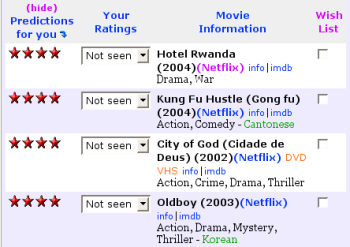
\includegraphics[scale=0.4]{img/movielens2}
\end{figure}

A cada avaliação, uma associação é feita entre as preferências de um usuário e as características do produto, que, neste exemplo, seriam as características dos filmes. Para um melhor compreendimento, ou para apresentar de uma maneira mais formal, podemos analisar a representação desta figura (Fig. 1) e de todo o sistema, representando todo os valores de avaliações em uma tabela formada, da mesma forma que foi ilustrado para exemplificar no algoritmo não personalizado, por usuários e por todos os itens que estão disponíveis para receber avaliações. Os dados encontrados são, a representação de todos os usuários, todos os itens e de todas as avaliações que já foram computadas, lembrando que, diferente da matriz utilizada no algoritmo não personalizado, a matriz na maioria das vezes é uma matriz esparsa, então podem existir poucas avaliações para determinado produto, ou um número não confiável de avaliações, podendo comprometer a recomendação, se não for utilizado, para a recomendação, uma técnica confiável, como o filtro colaborativo.


%{%
%\newcommand{\mc}[3]{\multicolumn{#1}{#2}{#3}}
%\begin{center}
%\begin{array} {ccccccc}
%× & \mc{6}{c}{\textit{Filmes}}\\\cline{2-7}
%\mc{1}{c|}{×} & \mc{1}{c|}{×} & \mc{1}{c|}{\textbf{1}} & \mc{1}{c|}{\textbf{2}} & \mc{1}{c|}{\textbf{3}} & \mc{1}{c|}{\textbf{4}} & \mc{1}{c|}{\textbf{5}}\\\cline{2-7}
%\mc{1}{c|}{×} & \mc{1}{c|}{\textbf{1}} & \mc{1}{c|}{?} & \mc{1}{c|}{?} & \mc{1}{c|}{?} & \mc{1}{c|}{?} & \mc{1}{c|}{5}\\\cline{2-7}
%\mc{1}{c|}{×} & \mc{1}{c|}{\textbf{2}} & \mc{1}{c|}{1} & \mc{1}{c|}{?} & \mc{1}{c|}{1} & \mc{1}{c|}{4} & \mc{1}{c|}{?}\\\cline{2-7}
%\mc{1}{c|}{\textit{Usuários}} & \mc{1}{c|}{\textbf{3}} & \mc{1}{c|}{?} & \mc{1}{c|}{3} & \mc{1}{c|}{?} & \mc{1}{c|}{?} & \mc{1}{c|}{?}\\\cline{2-7}
%\mc{1}{c|}{×} & \mc{1}{c|}{\textbf{4}} & \mc{1}{c|}{4} & \mc{1}{c|}{?} & \mc{1}{c|}{?} & \mc{1}{c|}{4.5} & \mc{1}{c|}{5}\\\cline{2-7}
%\mc{1}{c|}{×} & \mc{1}{c|}{\textbf{5}} & \mc{1}{c|}{?} & \mc{1}{c|}{2} & \mc{1}{c|}{3} & \mc{1}{c|}{?} & \mc{1}{c|}{?}\\\cline{2-7}
%\mc{1}{c|}{×} & \mc{1}{c|}{\textbf{6}} & \mc{1}{c|}{4} & \mc{1}{c|}{?} & \mc{1}{c|}{?} & \mc{1}{c|}{?} & \mc{1}{c|}{3}\\\cline{2-7}
%\end{array}
%\end{center}
%}%

Observando a matriz acima (ref da matriz), não é possível dizer, do ponto de vista humano, com facilidade quais são as referências e dizer todas as correlações existentes entre os valores dados como exemplo, logo, podemos afirmar que essa seria a primeira pergunta sobre como realizar a correlação entre os valores, dizendo o quão esses itens, ou usuários, são similares uns com os outros \cite{ricci2011introduction}, dependendo de qual aproximação foi adotada.

O filtro colaborativo é muito utilizado em sistemas web(colocar apud) \cite{turban2009electronic}, onde usuário podem repartir suas experiências com outros usuários sobre músicas, vídeos, livros ou qualquer outro produto, ou serviço, que possa receber alguma forma de avaliação, com o propósito de utilizar essas informações no futuro, sobre seus novos usuários. Além do uso para fins lucrativos, o filtro colaborativo é muito utilizado em sistemas de recomendação de diversos tipos de documentos, como trabalhos científicos, por exemplo \cite{sun2010new}. 

Para uma abordagem mais detalhada sobre o filtro colaborativo, os detalhes podem formar um melhor compreendimento sobre o assunto. Dentro dos detalhes, o filtro colaborativo é dividido em algumas principais aproximações, que são: a aproximação baseada nos usuários, a aproximação baseada nos itens. %(Posso falar também sobre), a aproximação baseada em históricos de usuários, e a aproximação baseada em modelo de aprendizagem \cite{asanov2011algorithms}\cite{su2009survey}. Exixtem diversos outras aproximações que não vão ser citadas aqui, como (Colocar as referências).


\subsubsection{Filtro colaborativo Baseado em Usuários}
Esta aproximação foi proposta por Jonathan L. Herlocker, professor da Universidade de Minnesota, no final da década de 90 \cite{sun2010new}. A aproximação baseada em usuários, como já comentado sobre isso alguns parágrafos acima, utiliza as avaliações dos usuários do sistema sobre determinado produto para recomendar esses produtos para outros usuários. Usuários que possuam grande similaridade de preferências são considerados, por conveniência de termos, como \textit{vizinhos}. Por tanto, um usuário que teve mais experiências com outros usuários que são seus \textit{vizinhos}, poderão receber recomendação partindo de suas preferências. O algoritmo baseado em \textit{usuários vizinhos} produz a sua predição de recomendação de determinado produto para outros usuários, utilizando o seu valor de avaliação que foi avaliado por seus \textit{usuários vizinhos}. Desta forma, podemos predizer avaliações de itens que ainda não foram avaliados \cite{zhao2010user}\cite{wang2006unifying}. 

Utilizando informações presentes em \cite{schafer2007collaborative}, podemos apresentar o algoritmo baseado em usuário de uma maneira mais formal. Por tanto, tomemos como exemplo um usuário $n$, que possui muitas similaridades com o usuário $u$, então podemos dizer que $n$ e $u$ são \textit{vizinhos}. Sendo $i$ um produto qualquer, sua avaliação pode ser obtida por outras avaliações de $i$ que foram efetuadas em momentos no passado por seu grupo de usuários que são \textit{vizinhos}. Além destas informações, é possível obter a média de todas as avaliações feitas por esta \textit{vizinhança}. Na equação seguinte, onde $r_ni$ é o valor de avaliação feita pelo seu \textit{vizinho} $n$, temos uma demonstração de como seria a predição nativa, representada por $pred$, do valor da avaliação de um produto $i$, para o usuário $u$, utilizando as avaliações feita por seu \textit{vizinho} $n$.

%equação 1 {pred(u,i)

É possível atingir a predição através da equação anterior, entretanto, seria necessário uma melhor aproximação, utilizando uma medida de avaliação de maior peso de quem for similar ao usuário $u$, ou seja, do seu \textit{vizinho}. Para isso, podemos tomar como exemplo uma função que calcula a similaridade entre $u$ e seu \textit{vizinho} $n$, que poderia ser chamada de $userSim(u,n)$, então a predição poderia ser feita utilizando a próxima formula. 

%equação 2 {pred(u,i)

Porém, caso o valor obtido pela função de similaridade não for maior do que um, a predição será obtida em escala incorreta. Para corrigir isso, podemo utilizar a função seguinte, onde o valor da equação anterior é dividido pelo valor da soma da similaridade dos \textit{vizinhos}.

%equação 3 {pred(u,i)

Tendo uma equação que consiga efetuar a predição dos valor para a recomendação, então já seria possível efetuar a recomendação baseada nos usuários do sistema. Um único inconveniente que poderia ainda persistir, seriam os usuários que possuam muitas variações em suas avaliações. Então, para recompensar essa variação, é possível utilizar a próxima função, que seria uma função de \textit{ajuste de média}.

%equanção 4

\subsubsection{Filtro Colaborativo Baseado em Itens}
Esta aproximação foi proposta por pesquisadores da Universidade de Minnesota durante pesquisas realizadas por volta do ano de 2001 \cite{sarwar2001item}. É possível afirmar que a aproximação por filtro colaborativo baseado em usuários é igualmente o oposto da aproximação por filtro colaborativo baseado em itens \cite{schafer2007collaborative}. O filtro colaborativo gera predição através da similaridade entre usuários, ditos \textit{vizinhos}, enquanto o filtro colaborativo baseado em itens gera sua predição por via da similaridade dos atributos dos itens dispostos no sistema. A aproximação por filtro colaborativo baseado em itens, utiliza como referência o fato de que as preferências dos usuários muda muito pouco e continua constante, formando, com os itens semelhantes, uma vizinhança de itens que são semelhantes. Por tanto, a recomendação poderá ser feita partindo de itens que estão presentes nesta vizinhança \cite{asanov2011algorithms}.

De forma análoga ao filtro colaborativo baseado em usuário, utilizando as informações das avaliações efetuadas por usuários que efetuaram avaliações e para todos os itens que receberam as avaliações, podemos recomendar novos itens para os usuários baseado nas preferências dos usuários, recomendando itens com similaridades e vizinhança de atributos. 

Para predizer os valores de avaliações que os itens receberam para a recomendação, é preciso calcular o quão similares os itens são uns com os outros. No âmbito da aproximação por filtro colaborativo baseado em itens, existem muitas variações da forma que a similaridade entre dois itens $(i, j)$ é calculada, como correlação de \textit{Pearson} (\textit{Pearson correlation}) \cite{herlocker2000understanding}, similaridade de co-seno (\textit{Cosine-based similarity}), similaridade de correlação (\textit{Correlation-based similarity}), similaridade de co-seno ajustado (\textit{Adjusted-cosine similarity}) \cite{sarwar2001item}, diferença do quadrado (\textit{mean-square difference}) \cite{shardanand1995social} e a \textit{Spearman Correlation} \cite{massa2004using}. A similaridade de co-seno ajustado (\textit{Adjusted-cosine similarity}), a mais popular, considerada por muitos também como a mais exata, métrica de similaridade é calculada utilizando todos os usuários que avaliaram ambos os itens $i$ e $j$. O valor resultante da equação da similaridade de co-seno ajustado (\textit{Adjusted-cosine similarity}) é obtido pela equação a seguir, onde $RB_ij$ $(rate both)$ é o conjunto de usuários que avaliaram ambos os itens $(i, j)$.

%equação itemSim(i,j)

Com o valor da similaridade dos itens, o peso do somatório das avaliações feitas pelo usuário $u$ sobre diversos itens similares a $i$ gera a predição para o usuário $u$ sobre o item $i$. Com a seguinte formula é possível realizar a predição.

%equação pred(u,i)

Observando a matriz de avaliações do filtro colaborativo baseado em usuários, a diferença entre ela e a matriz de avaliações do filtro colaborativo baseado em itens é que na aproximação baseada em usuários, os valores existente nas linhas são os valores utilizados para a predição, e na aproximação baseada em item, os valores existentes nas colunas são os valores utilizados para a predição \cite{sarwar2001item}. 


\subsubsection{Pontos fortes desta técnica}

\subsubsection{Pontos fracos desta técnica}


\subsection{Híbrido}
Existem diversas formas e variações sobre técnicas híbridas. A mais estudada é a fusão entre as técnicas de recomendação baseada em conteúdo e a recomendação por filtro colaborativo. Utilizando as duas predições, é possível, e mais provável, uma melhor precisão em pontos fracos dos dois algoritmos. Como a intenção é obter melhores resultados, a aproximação é realizada de forma separada, onde a técnica de recomendação baseada em conteúdo e a técnica de recomendação por filtro colaborativo predizem valores separadamente, e com os valores já encontrados, é possível realizar a fusão dos resultados, resultando em um vetor novo, que será o vetor resultado \cite{melville2010recommender}.

\subsubsection{Pontos fortes desta técnica}

\subsubsection{Pontos fracos desta técnica}

\subsection{Comparativo entre as técnicas abordadas}



\subsection{Subseção}


\chapter{O Problema}
\chapter{Considerações Finais}
Just-in-time

\bibliography{bib/bib}
\bibliographystyle{plain}

\end{document}